% -*- coding: utf-8 -*-
% !TEX encoding = UTF-8 Unicode
% !TEX root =  main.tex

\chapter{Beispiel Kapitel}
\label{chap:beispiel-kapitel}

In diesem Kapitel wird eine sehr kurze Einleitung in die Verwendung von \verb|LaTeX| beschrieben.\\
Für die Erstellung der Arbeit kann über \url{http://www.texstudio.org/} mit installierter TeX-Distribution \url{https://miktex.org/} das TeXstudio heruntergeladen werden. 

\section{Abbildungen}
Eine Abbildung lässt sich einfach über einfügen: \par\medskip

\lstset{language=TeX}
\begin{lstlisting}
\begin{figure}[h]
\centering
\includegraphics[width=\textwidth]{foc-ac-dc.pdf}
\caption{Beschriftung der Abbildung}
\label{fig:foc-ac-dc}
\end{figure}
\FloatBarrier
\end{lstlisting}

Die breite der Abbildung kann einerseits skaliert oder direkt im Maßstab von \SI{14.5}{\centi\meter} erstellt werden.
Wenn die Abbildung maßstabsgetreu erstellt wird, muss \verb|\centering| und der optionale Befehl \verb|[width=\textwidth]| nicht zwingend übernommen werden.\par\medskip

Es werden beim Auftreten des Befehls \verb|\FloatBarrier| alle bis dahin eingefügten Float-Umgebungen gesetzt Das kann z.B. dazu verwendet werden, dass Floats, wie figure oder table, nicht unterhalb einer neuen \verb|section| oder \verb|chapter| ausgegeben werden.\par\medskip

Abbildung \ref{fig:foc-dc-ac} zeigt \ldots \par\medskip

\begin{figure}[h]
	\centering
	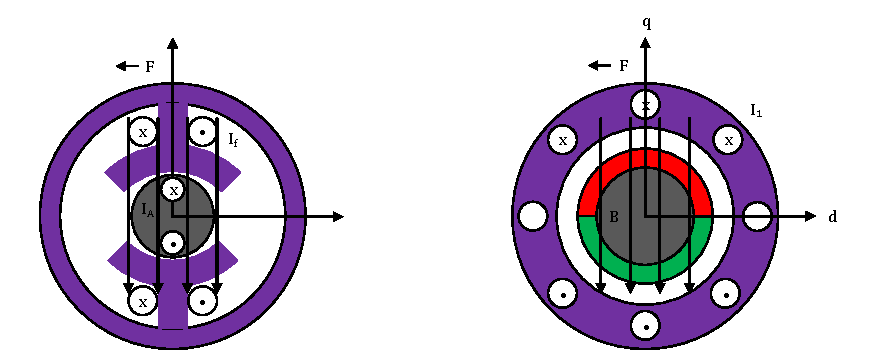
\includegraphics[width=\textwidth]{foc-dc-ac.pdf}
	\caption{Beschriftung der Abbildung}
	\label{fig:foc-dc-ac}
\end{figure}
\FloatBarrier

Durch setzten des \verb|[h]| hinter der \verb|figure| Umgebung, kann die Positionierung der Abbildung festgelegt werden.\par\medskip

Dabei sind folgende Werte ebenfalls möglich:

\begin{enumerate}
	\item h (here) - Gleicher Ort
	\item t (top) - Oben auf der Seite
	\item b (bottom) - Unten auf der Seite
	\item p (page) - Auf einer eigenen Seite
	\item ! (override) - Erzwingt die angegebene Position
\end{enumerate}

\section{Tabellen}\label{sec:tab}

Zur Erstellung einfacher Tabellen, bietet die Website \url{http://www.tablesgenerator.com/} eine einfach zu bedienende Oberfläche. \par\medskip %erzeugt einen mittleren Abstand

Für komplexere Tabellen können die \verb|multicol| und \verb|multirow| Pakete verwendet werden, wie in Tabelle \ref{tab:vgl_mosfet} dargestellt \cite{dalton}.
\begin{table}[h]
		\centering
	\renewcommand{\arraystretch}{1.6}
\begin{tabular}{lc|c|c|c|l}
	\cline{3-5}
	& \multicolumn{1}{l|}{} & \multicolumn{3}{c|}{MOSFET}             &  \\ \cline{3-5}
	& \multicolumn{1}{l|}{} & IRFS7530       & IPB019N08N3 & CSD19536KCS &  \\ \cline{3-5}
	& \multicolumn{1}{l|}{} & International Rectifier       & Infineon & Texas Instruments &  \\ \cline{1-5}
	
	\multicolumn{1}{|l|}{\multirow{4}{*}{\begin{turn}{90}Parameter\end{turn}}} & $Q_{\mathsf{G}}$                    &   354 \nano\coulomb             &  206 \nano\coulomb           &   153 \nano\coulomb      &  \\ \cline{2-5}
	\multicolumn{1}{|l|}{}                                                           & $Q_{\mathsf{GS}}$                   &  62 \nano\coulomb             &  50 \nano\coulomb          &  37 \nano\coulomb       &  \\ \cline{2-5}
	\multicolumn{1}{|l|}{}                                                           & $Q_{\mathsf{GD}}$                   & 73 \nano\coulomb              &  30 \nano\coulomb           &  17 \nano\coulomb       &  \\ \cline{2-5}
	\multicolumn{1}{|l|}{}                                                           & $R_{\mathsf{DSon}}$                 & 1,4 \milli\ohm & 1,9 \milli\ohm            &  3,5 \milli\ohm        &  \\ \cline{1-5}
\end{tabular}
	
	\caption{Vergleich verschiedener MOSFET \cite{dalton}}
	\label{tab:vgl_mosfet}
\end{table}
\FloatBarrier

\section{Zitate}\label{sec:cite}
Für Zitationen wird \verb|BibLaTeX| verwendet. Als Backend wird \verb|bibtex| vom Compiler verlangt.


\begin{quote}
\enquote{Bei jeder permanentmagneterregten Synchronmaschine ändern sich die Induktivitäten in Abhängigkeit von der Last. In erster Linie sind dafür die Sättigungseffekte, aber auch die Kreuzkopplung verantwortlich.} 
\end{quote}

Im Text zitierte Werke werden über die Syntax \verb|\textcite[S.~2]{ternes2015}| korrekt zitiert. Beispielsweise: Wie in \cite{ternes2015} erläutert, sind die Induktivitäten abhängig von der Last \ldots   \par\medskip

Der aktuelle Stil des Literaturverzeichnisses und der Zitationen ist \verb|IEEEtran|, kann aber auch in Absprache geändert werden, dazu empfiehlt es sich, die \verb|BibLaTeX|-Dokumentation zu konsultieren.\\
\clearpage
\section{Anhänge}\label{sec:Anhang}
Um Anhänge zu referenzieren, können diese mit Hilfe des  erstellten Anhangs (vgl. \ref{anhang_LastenheftEpOS}) referenziert werden.

\section{Formeln}\label{sec:Formeln}

Bei Implementierung von Formeln mit eingesetzten Werten, erweist sich eine Kombination von Tabelle und Formel als Sinnvoll. Tabelle \ref{tab:param_voltageDrop} zeigt die in Formel \ref{eq:voltagedrop} eingesetzten Parameter, mit Beschreibung sowie dem zugehörigen Wert \cite{drv8303}. \par\medskip

\begin{table}[h]
	\centering
	\begin{tabular}{ccc}
		\hline
		Parameter        &       Beschreibung        &           Wert           \\ \hline
		$V_{\mathsf{0}}$    & Maximale Ausgangsspannung &        3,3\ \volt        \\
		$V_{\mathsf{REF}}$   &     Referenz-Spannung     &        3,3\ \volt        \\
		$G$           &    Verstärkungsfaktor     & 40 $\frac{\volt}{\volt}$ \\
		${R}_{\mathsf{SHUNT}}$ &     Shunt-Widerstand      &    $500\ \micro\ohm$     \\ \hline
	\end{tabular}
	\caption{Parameter der Operationsverstärker-Einstellungen des DRV8303}
	\label{tab:param_voltageDrop}
\end{table}


\begin{equation}
\centering
V_{\mathsf{Smax}} = {\lvert ({SN}_{\mathsf{x}} - {SP}_{\mathsf{x}}) \rvert}_{\mathsf{max}} = \left( \frac{ \left({V}_{0} - \frac{ {V}_{\mathsf{REF}}}{2} \right)}{G}\right)   = 41,25\ \milli \volt
\label{eq:voltagedrop}
\end{equation}
\FloatBarrier

%%% Local Variables: 
%%% mode: latex
%%% TeX-master: "main"
%%% TeX-open-quote: "\\enquote{"
%%% TeX-close-quote: "}"
%%% LaTeX-csquotes-open-quote: "\\enquote{"
%%% LaTeX-csquotes-close-quote: "}"
%%% End: 
